\section{Architecture}
\label{sec:arch}

{\color{blue} Points to cover:

\begin{itemize}
    \item The goal: decode weak transmission by collating information from multiple base-stations
    \item Flow diagram (picture with cloudy and edgy stuff)
    \item The strawman comparison: stream everything
    \item Strawman limitations
        \begin{itemize}
            \item Weak signals and limited bandwidth (problems at gateways (could use joint decoding of preambles but cant afford to stream everything))
            \item Scaling issues (problems at the cloud)
        \end{itemize}
\end{itemize}
}


The goal of Charm is to decode weak transmissions, which could not be
decoded by any individual gateway, by collating receptions from multiple
gateways at the cloud. At one level, this  enables us to expand network coverage area reaching clients deep inside buildings, underground or in outer reaches of the city. More fundamentally, it saves energy on the vast majority of client devices, even if they are within range of some gateways, by allowing them to lower their transmit power without experiencing any loss in performance. 

The rest of this section describes the two key challenges in designing such an architecture: {\bf (1) At the Gateway: } First, given that signals from weak LP-WAN clients are often well below the noise floor (by as much as 37 dB), gateways are unaware of where these packets exist in the received signal. This means that base stations must effectively send all their received raw signal data to the cloud, stressing their limited uplink bandwidth. {\bf (2) At the Cloud: } Second, the cloud must identify signals from which gateways need to be combined over time to recover transmitted data. At city-scale, it is quite conceivable that overlapping weak transmissions from multiple LP-WAN clients are received at the same time by gateways, resulting in a challenging data recovery problem at the cloud. The rest of this section describes our solutions to each of these challenges. 

\subsection{Energy savings on client devices}

{\color{blue} describe the power argument here...}

\begin{figure}[!htb]
\centering
\begin{tabular}{@{}c@{}}	
\subfloat[Typical client device current consumption for a complete LoRaWAN transmission. The device is powered at $3V$.]{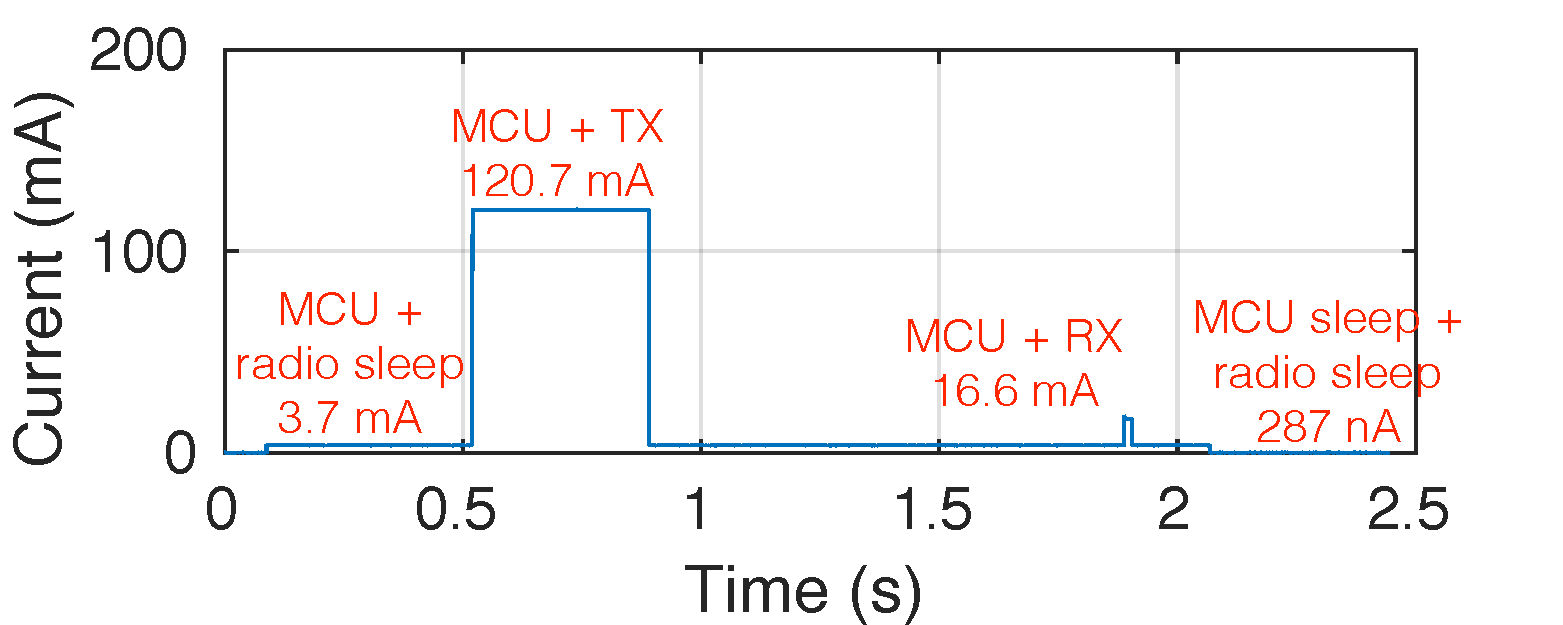
\includegraphics[width=0.4\textwidth]{figures/bug_power_trace_annotated}
\label{fig:power-trace}} \\
\subfloat[Estimated lifetime of a client device powered by two AA batteries at various bit rates based on energy profile.]{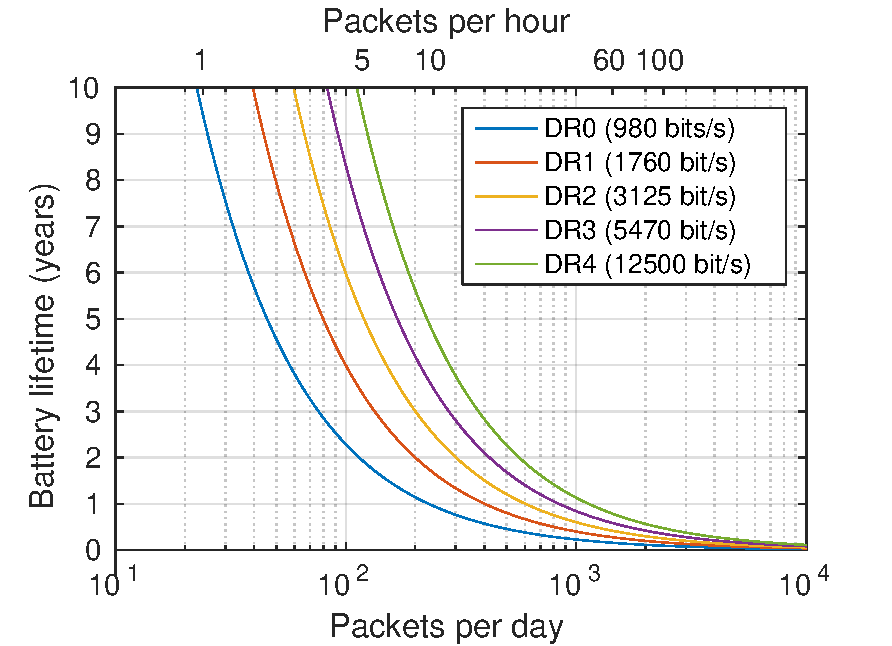
\includegraphics[width=0.4\textwidth]{figures/LoRaBug_AA_lifetime_semilog}
\label{fig:lifetime-estimates}}
\end{tabular}
\caption{}
\end{figure}

\begin{figure}[!ht]
\centering
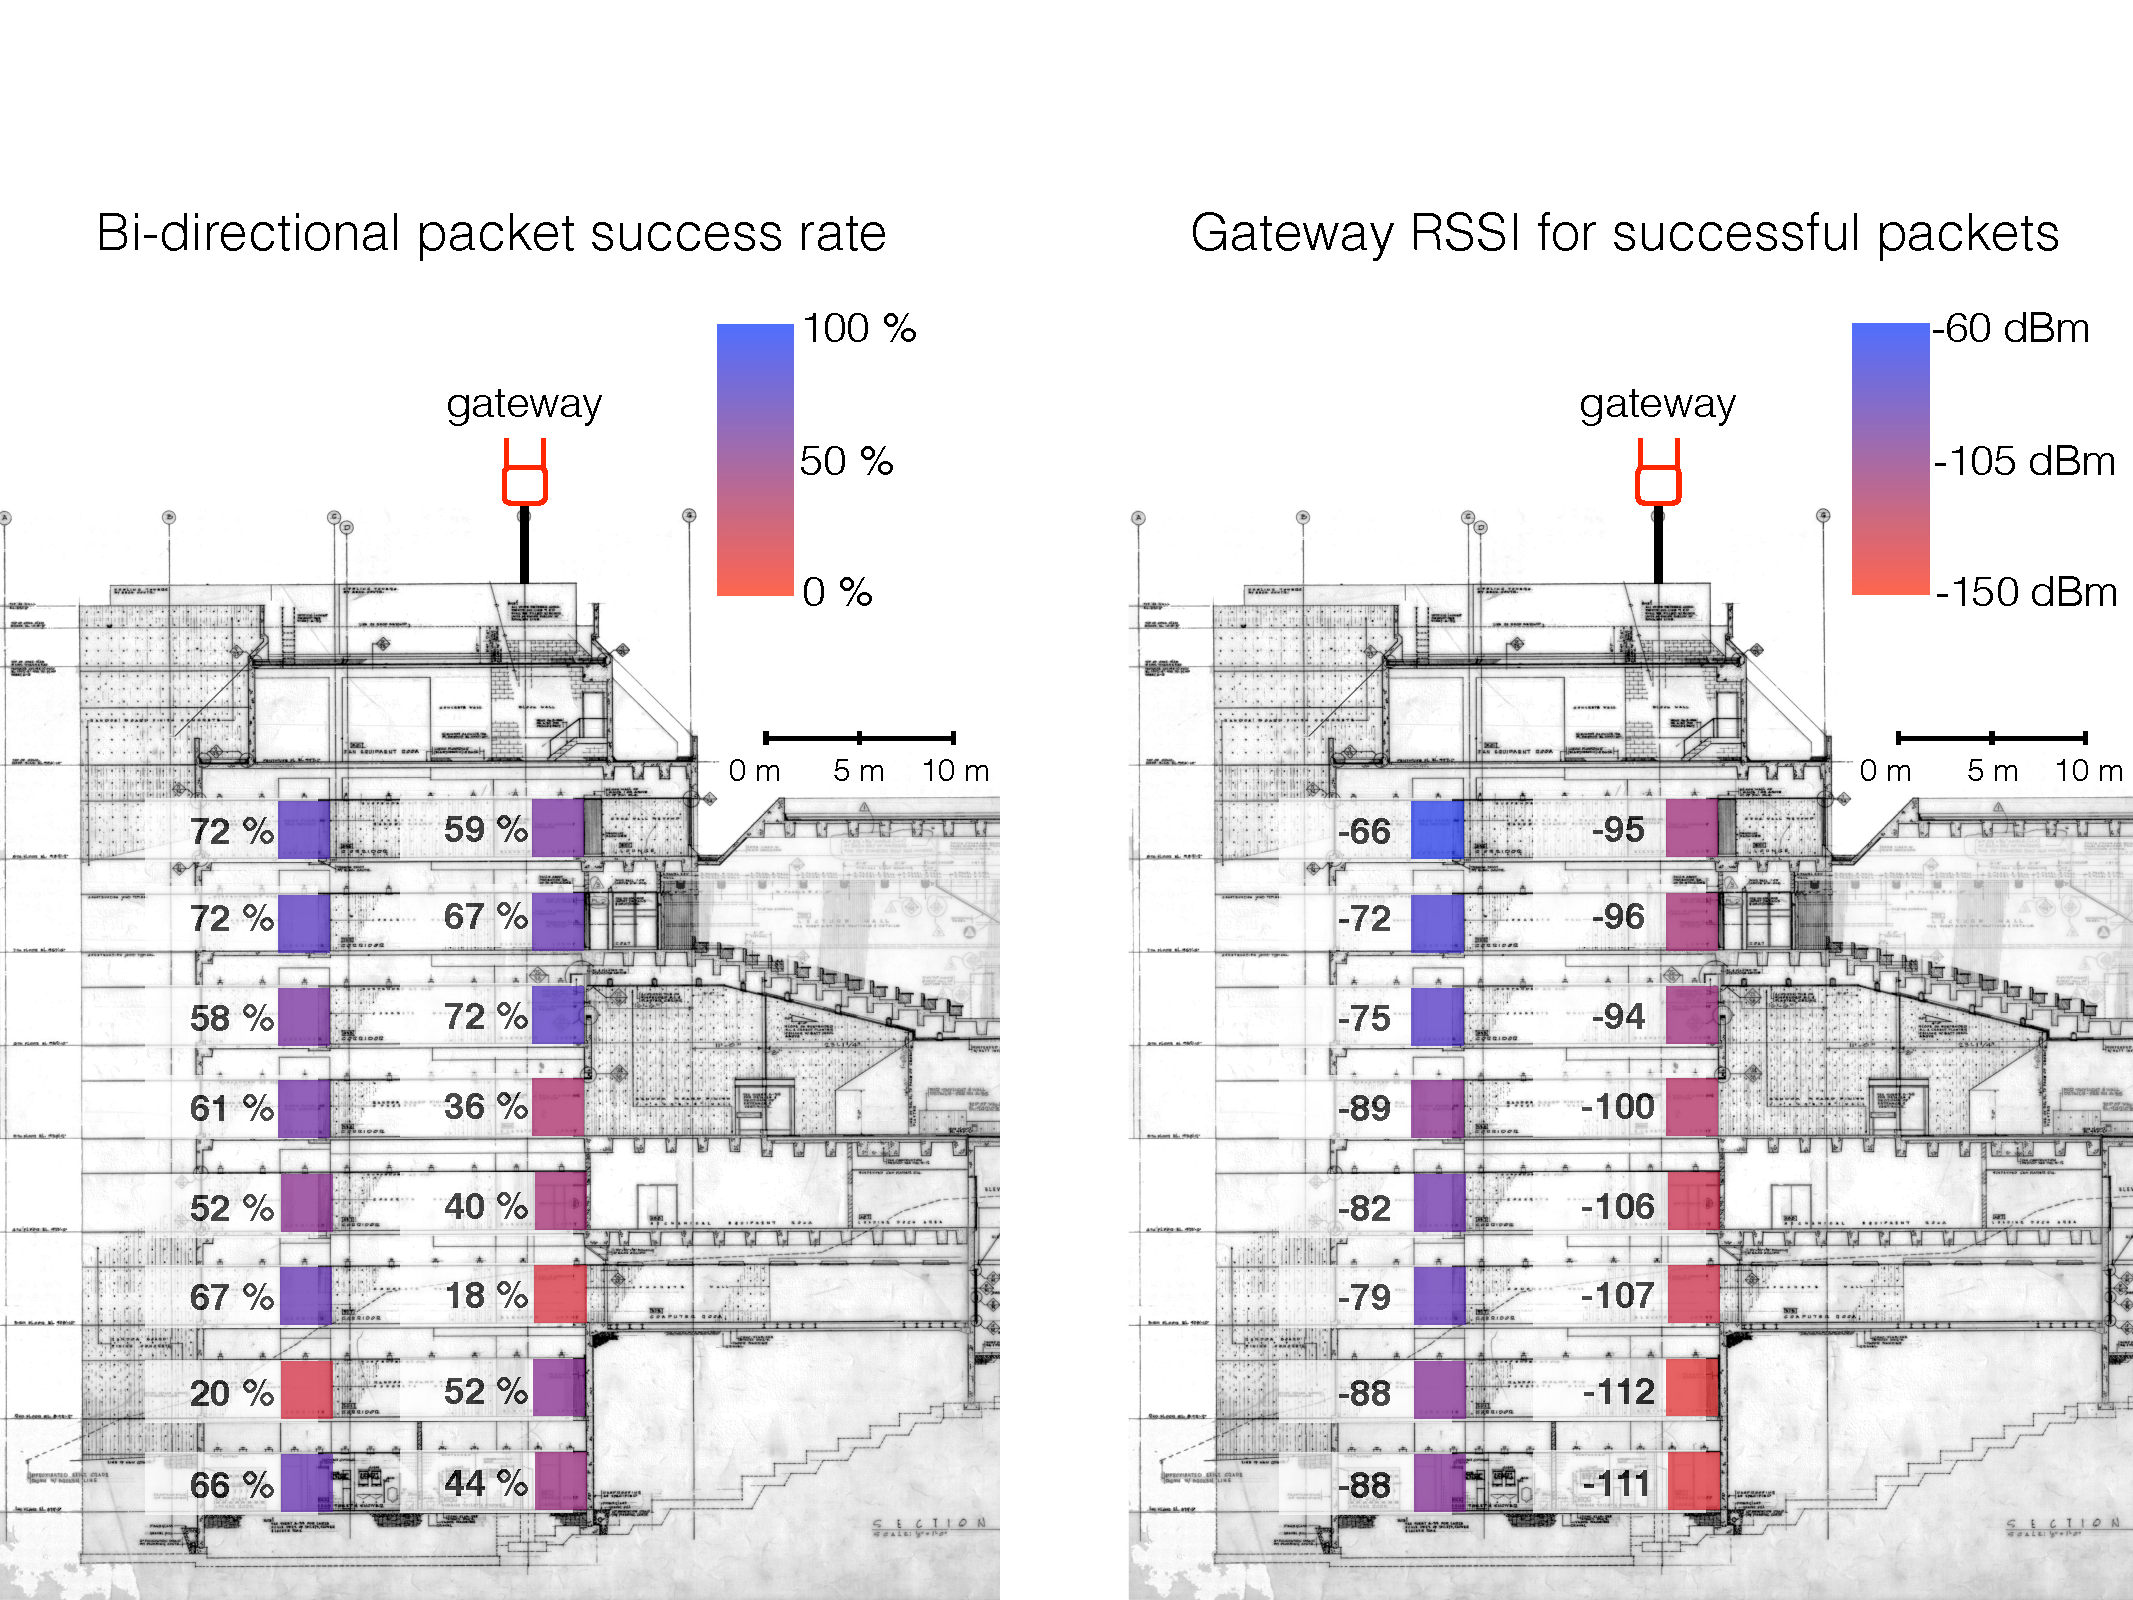
\includegraphics[width=0.5\textwidth]{figures/penetration_test_wean_cropped}
\compactimg
\caption{RF signal penetration experiments performed in a large poured-concrete building. (Left) shows the success rate for bi-directional packet exchange between end-node and gateway and (right) shows the RSSI at the gateway for successful transfers.}
\label{fig:penetration-test}
\end{figure}

Some of the transmission our system aims to decode, have signal power as low
as -30 dBm below the noise floor. Such transmission are not only impossible to
decode for an individual gateway, but they are also difficult to detect .
Since transmitted signals would combine coherently, contrasted to random noise
that combines non-coherently, an appropriate combination of radio streams
from different gateways might be able to decode such a message.

\subsection{Continuous streaming}
\label{sec:continuus-streaming}

A solution, similar to Cloud-RAN \cite{chen2011c}, is to continuously
stream all radio data to a cloud-based joint decoder. The gateways then act as
simple forwarders while all decisions and processing is done by a capable and
scaleable cloud server. This architecture is similar to LoRaWAN, but for the
physical layer. Additionally, joint detection of packets might detect even
weaker packets that what is detectable by a single receiver.

However, streaming raw radio I/Q data streams to the cloud at each base
station suffers from two major issues: (1) They require high bandwidth
connectivity between gateways and the cloud decoder -- typically a fiber-optic
backhaul. Indeed, streaming LoRaWAN raw signal data at its lowest bandwidth
to the cloud would incur 18 Mbps of uplink bandwidth. This is far too
expensive and wasteful, given the limited uplink bandwidth at
consumer-deployed LoRaWAN gateways which are often just home set-top boxes.
(2) Processing large amounts of data at the cloud poses a scalability
challenge with an increasing number of gateways.

%2.250 MBps

% Swarun



% {\color{blue} Describe the entire story in this section}

Note: continuous streaming data rate 2.250 MBps for 8 channel gateways

\subsection{Selective aggregation}
\label{sec:selective-aggregation}

A: LoRa packets have this nice characteristic of having a very long header. We could detect packets locally and only stream detected chunks to the cloud

Q: Our network is very vast and performance degrades near the boundaries, which also cover the most area. At any point of time there will always be many struggling transmitters.
